
\documentclass[11pt]{article}
\usepackage[margin=1in]{geometry}
\usepackage{graphicx}
\usepackage{amsmath,amssymb}
\usepackage{booktabs}
\usepackage{tabularx}
\usepackage{float}
\usepackage{hyperref}
\usepackage{xurl}
\usepackage[numbers,sort&compress]{natbib}
\usepackage{caption}
\usepackage{setspace}
\usepackage[T1]{fontenc}
\hypersetup{colorlinks=true,linkcolor=black,citecolor=black,urlcolor=blue}
\setstretch{1.12}
\sloppy
\emergencystretch=3em
\Urlmuskip=0mu plus 2mu

\title{Claim-Bounded Diagnostics for Noise-Assisted Annealing and Frustration Boundaries in an Information-Feedback Active-Particle Surrogate\\\large Integrated Model, Reconstructed ABP Diagnostics, and v0.2.x Audit Synthesis}
\author{Keiji Yoshimura\\\small Independent Researcher}
\date{May 25, 2026\\\small v0.3.1 Integrated Revision}

\begin{document}
\maketitle

\begin{center}
\small
GitHub repository: \url{https://github.com/yokken0907/active-particle-feedback-kinetic-arrest}\\
License: source-defined Evaluation-Only Notice in the repository.\\
Historical repository archive DOI: \href{https://doi.org/10.5281/zenodo.20202120}{10.5281/zenodo.20202120}.
\end{center}

\begin{abstract}
This integrated revision combines the earlier ABP-style manuscript on kinetic-arrest-like behavior and noise-induced annealing with the subsequent v0.2.0--v0.2.6 claim-boundary audit sequence. The original manuscript introduced an active-particle surrogate with positional dynamics, orientational alignment, internal attributes, and a local variance-minimizing information-feedback update. Reconstructed diagnostics showed finite-size order-parameter and susceptibility motifs together with spatial-correlation recovery under moderate noise. The later audit sequence substantially narrows the interpretation. Within the implemented toy-model setting, a noise-assisted annealing window was observed across multiple tested conditions, and local feedback was sometimes competitive or beneficial relative to null controls. However, the effect was not uniquely attributable to local feedback, and high-frustration geometries produced first-class failure boundaries. By v0.2.6, formerly persistent boundaries split into rescue-stable and persistent-hard-boundary regimes under targeted relief, with extreme frustration remaining unrecovered in the tested setting. This paper does not claim experimental active-matter validation, biological or social-system validation, crowd-control or civilization-engineering interpretation, a universal kinetic-arrest mechanism, or local feedback as a uniquely necessary annealing generator.
\end{abstract}

\paragraph{Reader guidance and claim boundary.}
This manuscript should be read as a reduced active-particle surrogate diagnostic. It is adjacent to collective-motion and active-matter modeling, including Vicsek-type self-driven particles \cite{vicsek1995}, Toner--Tu flocking theory \cite{toner1998}, active-matter hydrodynamics \cite{marchetti2013}, and active particles in complex environments \cite{bechinger2016}. It also uses kinetic-arrest-like, clustering, and phase-separation language only as bounded surrogate vocabulary, with nearest conceptual background in motility-induced phase separation and phase-separating active colloids \cite{cates2015,fily2012,redner2013}. The allowed claims are limited to model-internal noise-window diagnostics, feedback-geometry dependence, frustration-boundary classification, and rescue-stability behavior inside the tested toy-model setting.

\section{Introduction}
Active matter systems consist of elements that autonomously generate propulsive forces and can display collective organization far from equilibrium. Since the Vicsek model \cite{vicsek1995}, theoretical and numerical work has shown that simple local interactions can generate transition-like collective motion, symmetry breaking, and scale-dependent fluctuations. Continuum theories and reviews of active matter provide a broad modeling background for such systems \cite{toner1998,marchetti2013,bechinger2016}.

The present surrogate asks a narrower question: what diagnostic motifs appear when active particles carry internal attributes and are subject to local information-feedback dynamics that tends to reduce local attribute variance? The initial hypothesis was that competing active motion, volume exclusion, local optimization, and feedback-mediated alignment of internal attributes might generate kinetic-arrest-like fragmentation at low noise, while moderate noise might assist escape from metastable local domains. That early framing produced a useful model narrative, but it was still too strong if read as a universal physical or social interpretation.

The later v0.2.x audit sequence therefore reframed the work as a claim-boundary exercise. Rather than asking only whether a positive annealing-like phenomenon could be shown, the audit asked whether feedback was necessary, whether a frozen noise window generalized, whether high-frustration geometries failed, whether targeted rescue generalized, and whether persistent hard boundaries remained. This integrated manuscript preserves the model and baseline reconstructed diagnostics from the earlier paper, while replacing the stronger interpretation with the more conservative v0.3.1 synthesis.

\section{Model}
Consider a system of $N$ active particles moving in two-dimensional periodic boundary conditions with system size $L \times L$. Each particle $i$ has position $\mathbf{r}_i$, orientation angle $\theta_i$, and scalar internal attribute $q_i \in [-1,1]$. The translational update is written as
\begin{equation}
\frac{d\mathbf{r}_i}{dt} = v_0 \mathbf{n}_i + \mathbf{F}^{\mathrm{rep}}_i + \mathbf{F}^{\mathrm{attr}}_i + \boldsymbol{\xi}^{\mathrm{tr}}_i(t),
\end{equation}
where $\mathbf{n}_i=(\cos\theta_i,\sin\theta_i)$ and $\boldsymbol{\xi}^{\mathrm{tr}}_i(t)$ denotes translational noise.

Short-range repulsion is represented by a Weeks--Chandler--Andersen-type potential \cite{weeks1971},
\begin{equation}
U_{\mathrm{WCA}}(r) =
\begin{cases}
4\epsilon\left[ \left(\dfrac{\sigma}{r}\right)^{12} - \left(\dfrac{\sigma}{r}\right)^6 \right] + \epsilon, & r < 2^{1/6}\sigma,\\
0, & r \ge 2^{1/6}\sigma.
\end{cases}
\end{equation}
The internal-attribute-dependent interaction is written as
\begin{equation}
U_{\mathrm{attr}}(r_{ij};q_i,q_j) = -Jq_iq_j\frac{e^{-\kappa r_{ij}}}{r_{ij}+a},
\end{equation}
with force $\mathbf{F}^{\mathrm{attr}}_i=-\sum_{j\ne i}\nabla_i U_{\mathrm{attr}}(r_{ij};q_i,q_j)$.

The orientation evolves through local alignment and angular noise,
\begin{equation}
\frac{d\theta_i}{dt}=\lambda_{\mathrm{align}}\sin(\Theta_i-\theta_i)+\eta_i(t),
\end{equation}
where $\Theta_i=\mathrm{Arg}(\sum_{j\in\mathcal{N}_i}\mathbf{n}_j)$ is the neighborhood mean direction. The internal attribute update is
\begin{equation}
\frac{dq_i}{dt}= -\lambda_{\mathrm{int}}(q_i-\langle q\rangle_R) - \chi q_i(q_i^2-1)+\zeta_i(t),
\end{equation}
where the first term is interpreted as local variance-minimizing information feedback and the second term keeps the scalar attribute within a bounded bistable range. Numerical integration in the reconstructed baseline used Euler--Maruyama-style discretization \cite{maruyama1955}, with finite-size checks over $N\in\{64,128,256\}$ in the public diagnostic reconstruction.

\section{Reconstructed baseline diagnostics}
The earlier manuscript reported reconstructed public diagnostics rather than a complete bit-level replay of every exploratory local run. The global orientational order parameter and susceptibility were defined as
\begin{equation}
\Phi = \left| \frac{1}{N}\sum_{j=1}^{N} e^{i\theta_j}\right|, \qquad \chi_\Phi = N\mathrm{Var}(\Phi).
\end{equation}
Figure~\ref{fig:baseline_order} summarizes the finite-size diagnostic. The original interpretation was that low-noise conditions could produce a decrease in global order with a susceptibility motif suggestive of kinetic-arrest-like fragmentation. In the present integrated revision, this is treated as a reconstructed diagnostic motif, not as proof of a universal kinetic-arrest transition.

\begin{figure}[H]
\centering
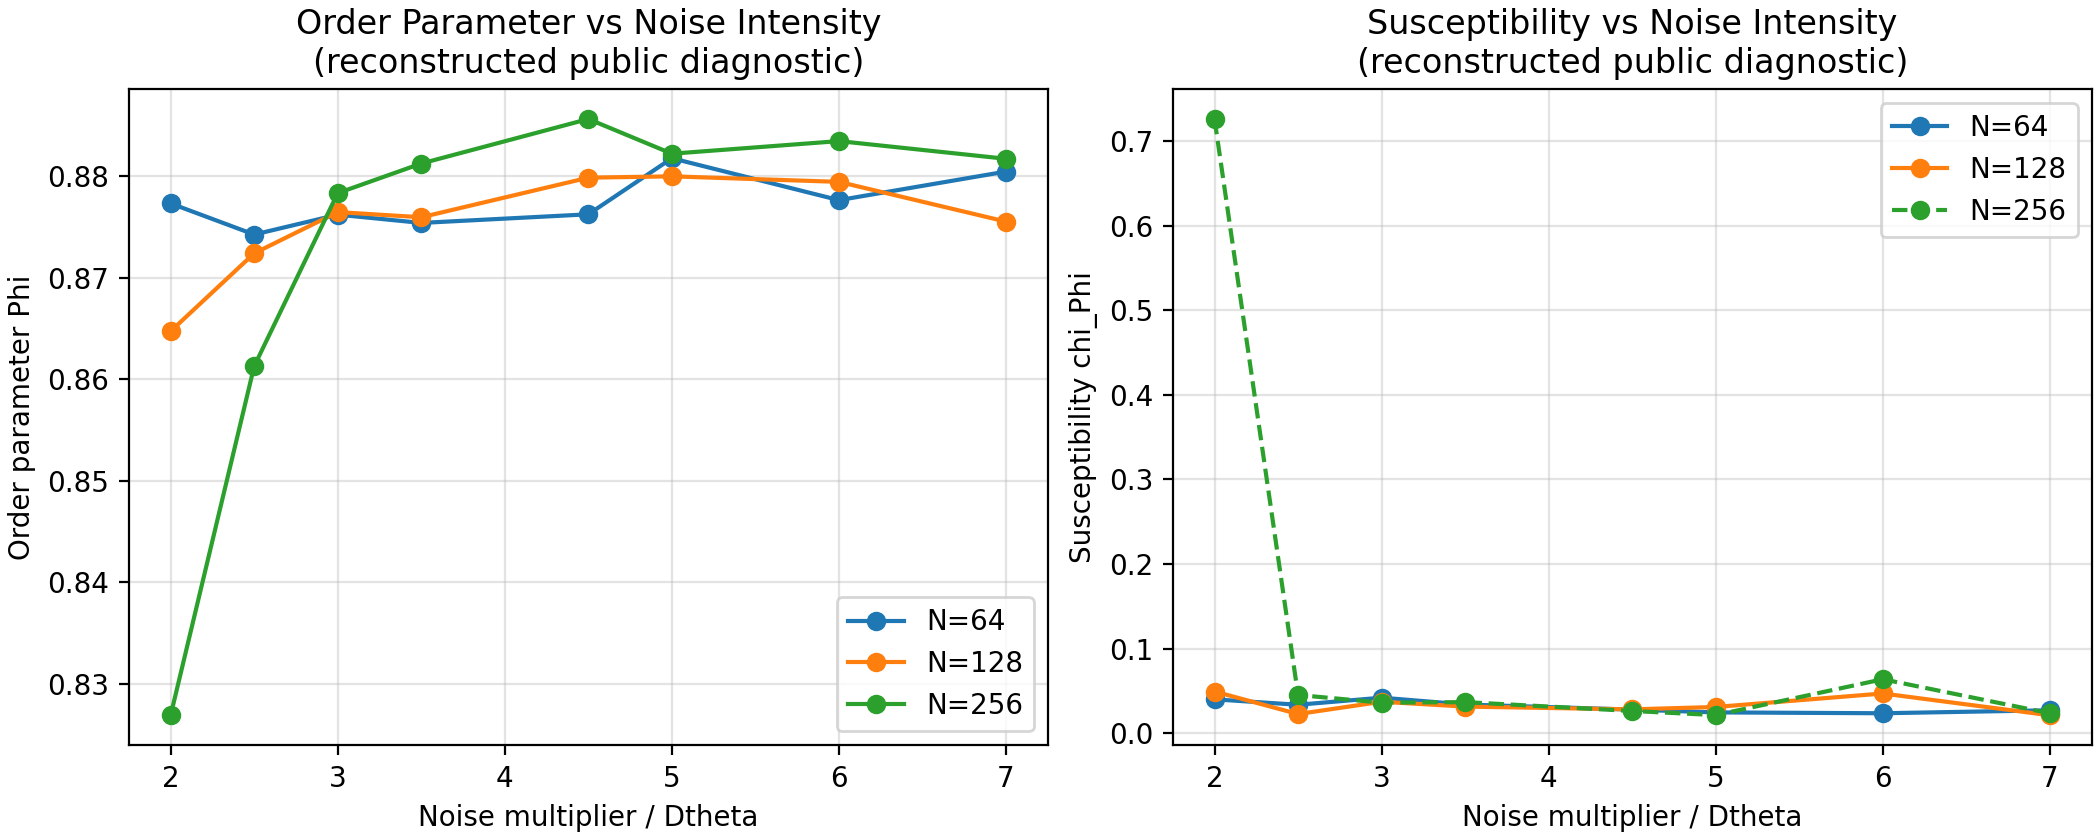
\includegraphics[width=0.86\linewidth]{figure1_order_susceptibility_reconstructed.png}
\caption{Reconstructed finite-size diagnostic for the baseline active-particle feedback surrogate. The figure is retained from the earlier manuscript as a model-internal diagnostic of order and susceptibility motifs, not as an experimental active-matter validation.}
\label{fig:baseline_order}
\end{figure}

The spatial-correlation diagnostic was defined in terms of an orientational correlation function $C(r)=\langle\mathbf{n}_i\cdot\mathbf{n}_j\rangle_{|\mathbf{r}_i-\mathbf{r}_j|=r}$. Figure~\ref{fig:baseline_corr} shows the reconstructed comparison between a lower-noise and a more moderate-noise condition. The safe interpretation is that moderate noise can improve long-range correlation in this reduced implementation, consistent with a noise-assisted relaxation or annealing-window hypothesis. It does not establish that feedback control uniquely produces such a window.

\begin{figure}[H]
\centering
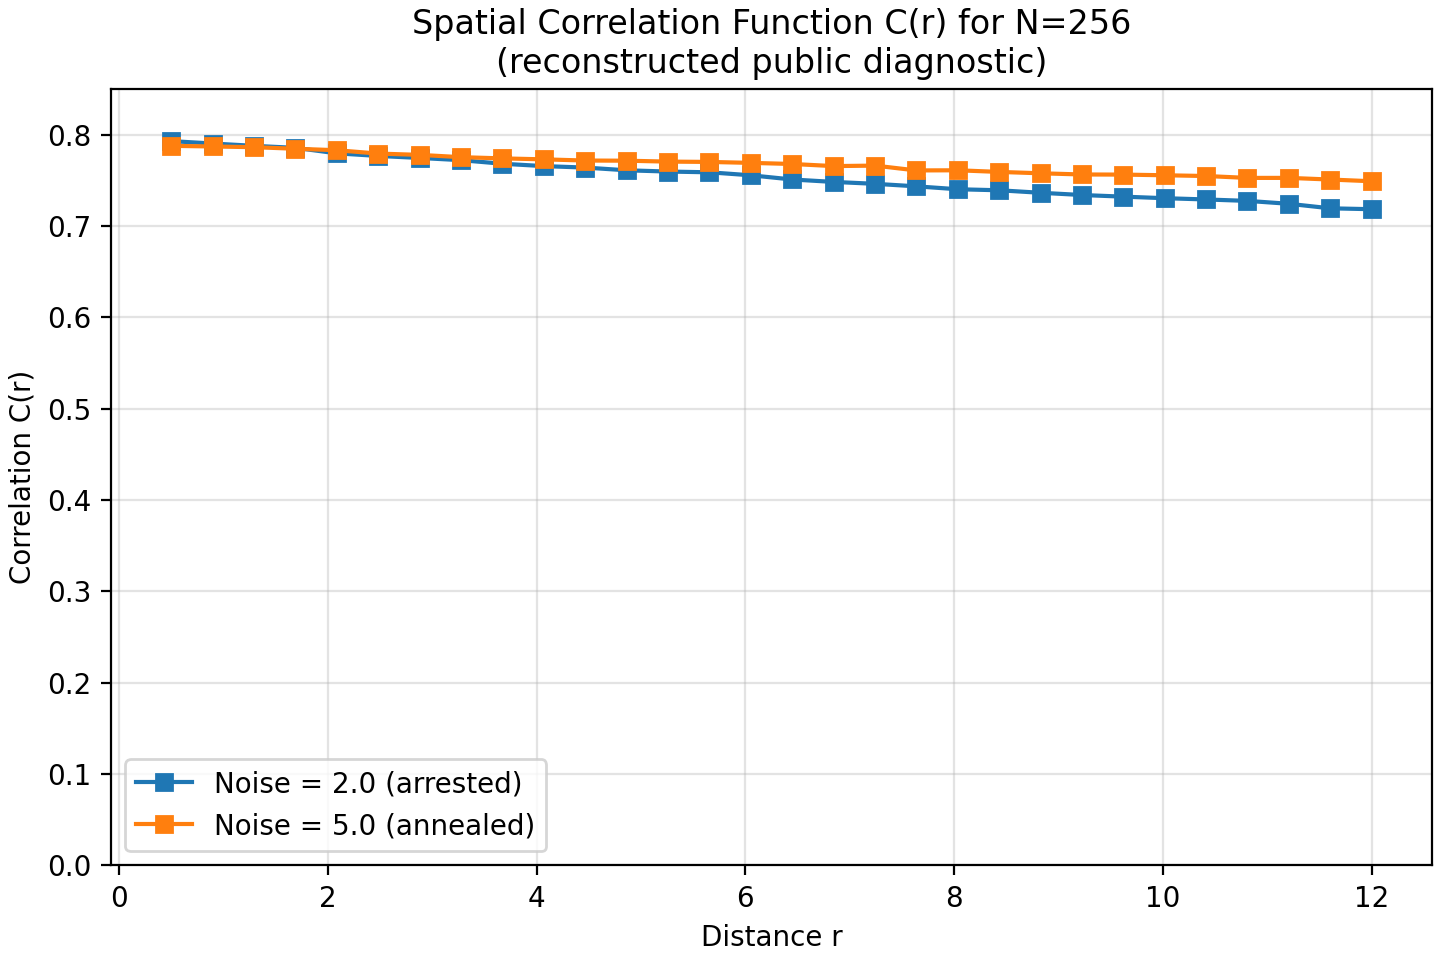
\includegraphics[width=0.76\linewidth]{figure2_spatial_correlation_reconstructed.png}
\caption{Reconstructed spatial-correlation diagnostic. The comparison motivates the noise-assisted annealing-window hypothesis while remaining limited to the reduced surrogate.}
\label{fig:baseline_corr}
\end{figure}

\section{Extended audit sequence}
The v0.2.0--v0.2.6 audit sequence tested whether the baseline interpretation survived controls, holdout geometries, and failure-boundary checks. Table~\ref{tab:phase_ledger} summarizes the integrated reading.

\begin{table}[H]
\centering
\caption{Condensed v0.2.x audit ledger used in the v0.3.1 integrated revision.}
\label{tab:phase_ledger}
\begin{tabularx}{\linewidth}{p{0.16\linewidth}p{0.30\linewidth}X}
\toprule
Phase & Main audit & Integrated reading\\
\midrule
v0.2.0 & Arrest/annealing/ablation preflight & A noise-assisted annealing window appeared, but feedback-mediated fragmentation was not stably locked.\\
v0.2.1 & Mechanism disambiguation & Local feedback was not uniquely responsible for the window; controls remained important.\\
v0.2.2 & Topology/noise holdout & Annealing windows appeared across several tested conditions, including controls.\\
v0.2.3 & Frozen-window holdout & Local feedback became competitive and often advantageous, but positive windows also remained in null controls.\\
v0.2.4 & Frustration rescue & High-frustration geometries produced native failures that could be rescued in tested settings.\\
v0.2.5 & Frozen rescue holdout & Some rescue effects generalized, but several persistent failure boundaries remained.\\
v0.2.6 & Persistent-boundary classification & Most boundaries were rescue-stable, while extreme frustration remained a persistent hard boundary.\\
\bottomrule
\end{tabularx}
\end{table}

Figure~\ref{fig:frozen_window} shows the frozen-window score comparison from the holdout stage. This result is important because it strengthens the case that local feedback can be competitive in some geometries, without requiring the stronger claim that local feedback is the unique cause of the annealing window.

\begin{figure}[H]
\centering
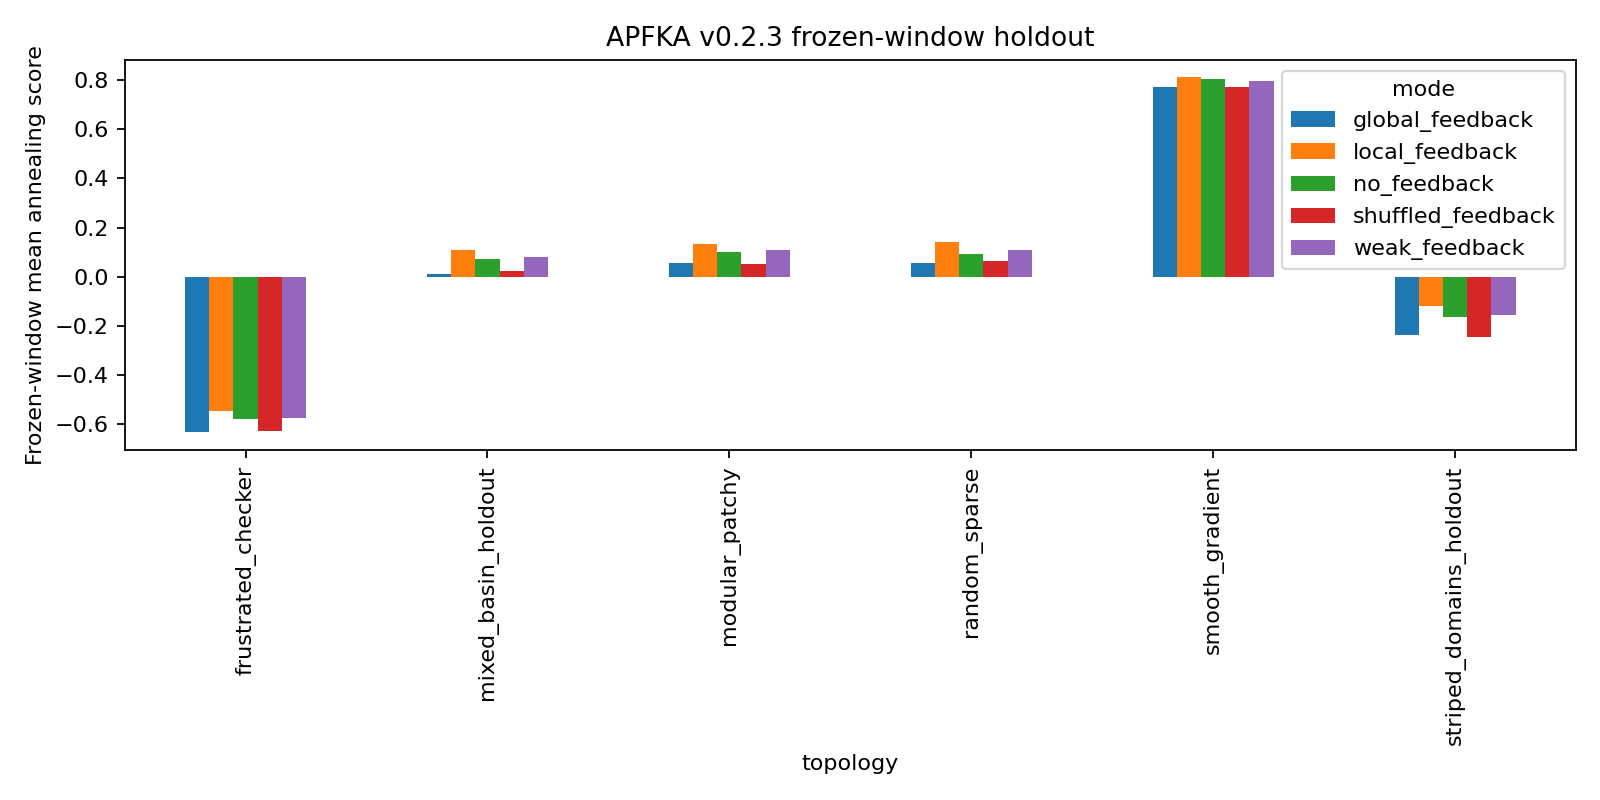
\includegraphics[width=0.86\linewidth]{v0_2_3_apfka_v023_frozen_window_scores.png}
\caption{Frozen-window holdout comparison from v0.2.3. Local feedback was often competitive, but the window itself was not uniquely attributable to local feedback.}
\label{fig:frozen_window}
\end{figure}

\section{Frustration boundary and rescue classification}
The terminal v0.2.6 audit classified boundary behavior after targeted interventions. It recorded four native failure boundaries, seven rescue-stable classifications, no conditional-rescue cases, and one persistent hard boundary. The mean native local-minus-no-feedback score was 0.1254227, while the mean best-minus-native gain on native failures was 1.2053399. Table~\ref{tab:terminal_boundary} gives the terminal boundary classification.

\begin{table}[H]
\centering
\caption{Terminal v0.2.6 boundary classification. Scores are dimensionless surrogate diagnostics.}
\label{tab:terminal_boundary}
\begin{tabularx}{\linewidth}{Xrrl}
\toprule
Topology & Native & Best & Classification\\
\midrule
extreme frustration holdout & -1.5878 & -0.8117 & persistent hard boundary\\
frustrated checker phase shift & -1.1662 & 0.2224 & rescue stable\\
frustrated checker v2 & -0.8548 & 0.5698 & rescue stable\\
striped domains holdout v2 & -0.2875 & 0.9446 & rescue stable\\
mixed basin holdout v2 & 0.8781 & 1.1916 & rescue stable\\
modular patchy holdout & 1.0555 & 1.3201 & rescue stable\\
random sparse holdout & 0.8849 & 1.1438 & rescue stable\\
smooth gradient holdout & 0.5135 & 0.8354 & rescue stable\\
\bottomrule
\end{tabularx}
\end{table}

\begin{figure}[H]
\centering
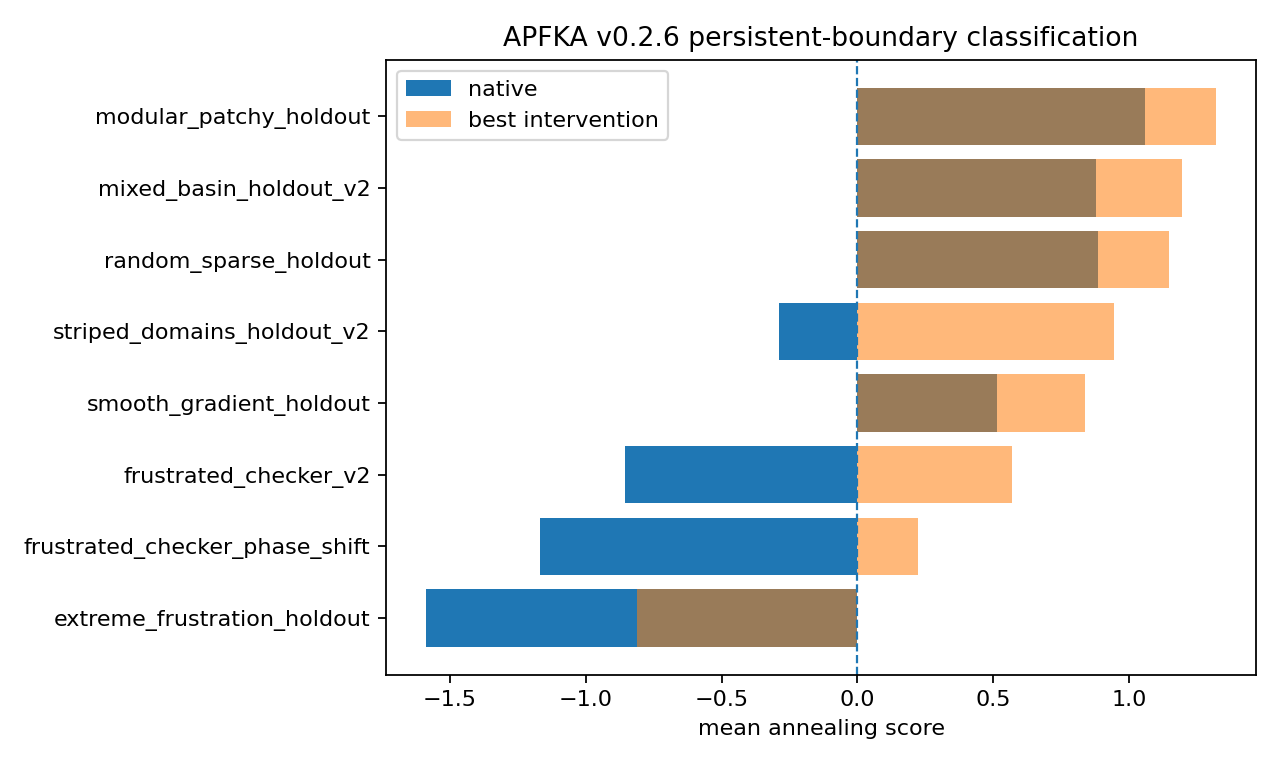
\includegraphics[width=0.86\linewidth]{v0_2_6_apfka_v026_boundary_scores.png}
\caption{Terminal boundary-score comparison from v0.2.6. The separation between rescue-stable and persistent-hard-boundary regimes is a model-internal diagnostic result.}
\label{fig:boundary_scores}
\end{figure}

\begin{figure}[H]
\centering
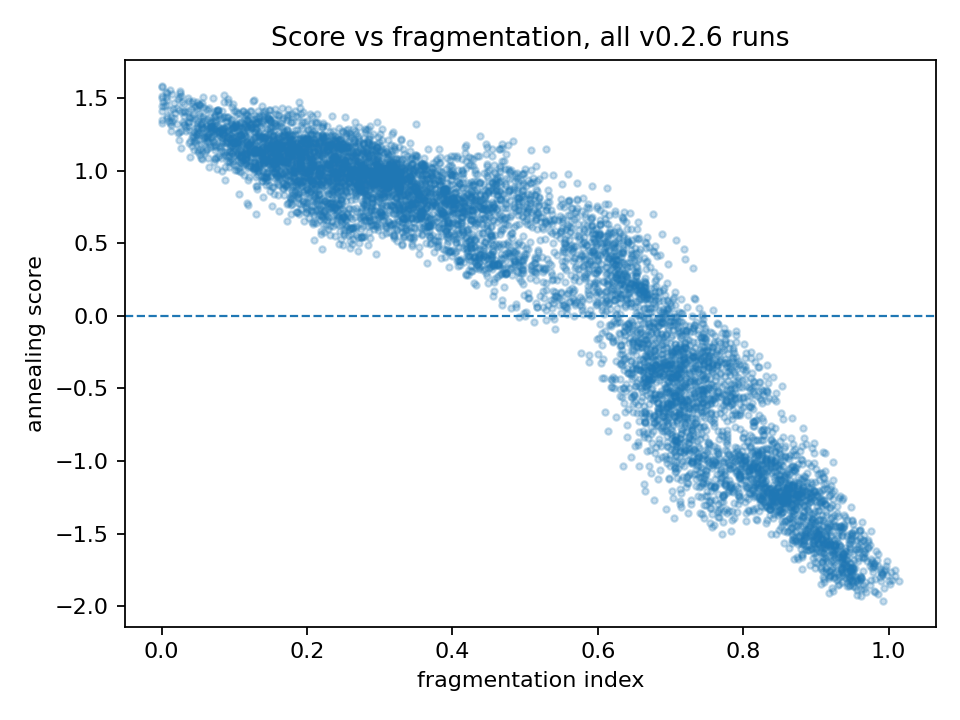
\includegraphics[width=0.86\linewidth]{v0_2_6_apfka_v026_score_vs_fragmentation.png}
\caption{Score-fragmentation diagnostic from the terminal boundary classification. The pattern supports a surrogate-level classification of frustration and rescue stability inside the tested implementation.}
\label{fig:score_fragmentation}
\end{figure}

\section{Integrated interpretation}
The integrated interpretation is narrower than both the original broad metaphor and the strongest reading of the initial ABP diagnostics. The preserved positive result is a noise-assisted relaxation or annealing-window motif in a reduced active-particle surrogate. The preserved feedback result is that local feedback can be competitive and sometimes beneficial relative to null controls. The negative result is equally important: annealing-window behavior is not uniquely attributable to local feedback, and high-frustration geometries can remain unrecovered even after targeted relief.

This resolves the tension between the older, richer manuscript and the shorter v0.3.0 synthesis addendum. The older text supplied the model, equations, numerical-diagnostic narrative, and scientific neighborhood. The v0.2.x audits supplied the necessary claim boundary: the object is not a universal feedback-induced kinetic-arrest theory, but a structured diagnostic of noise windows, feedback geometry, frustration boundaries, rescue stability, and persistent hard boundaries.

\section{Limitations}
The following interpretations are explicitly excluded. This manuscript does not claim experimental validation in active matter, biological validation, social-system validation, crowd-control or swarm-control deployment, civilization-engineering guidance, policy applicability, a universal kinetic-arrest theorem, or proof that local feedback is necessary for noise-induced annealing. The figures and tables are diagnostic artifacts of the implemented reduced surrogate. The historical repository DOI is a repository-archive identifier, not a peer-reviewed article DOI and not a validation certificate.

\section*{Data and code availability}
The repository is available at \url{https://github.com/yokken0907/active-particle-feedback-kinetic-arrest}. The historical repository archive DOI \href{https://doi.org/10.5281/zenodo.20202120}{10.5281/zenodo.20202120} is retained as repository-archive context. Zenodo identifiers generated for repository releases should be interpreted as repository archive DOIs rather than standalone peer-reviewed article DOIs. The package includes the reconstructed public ABP reproducer, the v0.2.x audit evidence, selected figures, file manifests, claim-boundary documentation, and this integrated revision.

\section*{Conflict of interest}
The author declares no institutional, financial, or commercial conflict of interest related to this study.

\section*{AI assistance disclosure}
The author used AI assistance for drafting, code generation, numerical-audit scaffolding, and manuscript preparation. The author remains responsible for the final claim boundary, interpretation, and release decisions.

\begin{thebibliography}{99}
\bibitem{vicsek1995} T. Vicsek, A. Czirok, E. Ben-Jacob, I. Cohen, and O. Shochet, ``Novel Type of Phase Transition in a System of Self-Driven Particles,'' \emph{Physical Review Letters}, 75, 1226--1229, 1995. DOI: \href{https://doi.org/10.1103/PhysRevLett.75.1226}{10.1103/PhysRevLett.75.1226}.
\bibitem{toner1998} J. Toner and Y. Tu, ``Flocks, herds, and schools: A quantitative theory of flocking,'' \emph{Physical Review E}, 58, 4828--4858, 1998. DOI: \href{https://doi.org/10.1103/PhysRevE.58.4828}{10.1103/PhysRevE.58.4828}.
\bibitem{marchetti2013} M. C. Marchetti et al., ``Hydrodynamics of soft active matter,'' \emph{Reviews of Modern Physics}, 85, 1143--1189, 2013. DOI: \href{https://doi.org/10.1103/RevModPhys.85.1143}{10.1103/RevModPhys.85.1143}.
\bibitem{bechinger2016} C. Bechinger et al., ``Active particles in complex and crowded environments,'' \emph{Reviews of Modern Physics}, 88, 045006, 2016. DOI: \href{https://doi.org/10.1103/RevModPhys.88.045006}{10.1103/RevModPhys.88.045006}.
\bibitem{cates2015} M. E. Cates and J. Tailleur, ``Motility-Induced Phase Separation,'' \emph{Annual Review of Condensed Matter Physics}, 6, 219--244, 2015. DOI: \href{https://doi.org/10.1146/annurev-conmatphys-031214-014710}{10.1146/annurev-conmatphys-031214-014710}.
\bibitem{fily2012} Y. Fily and M. C. Marchetti, ``Athermal Phase Separation of Self-Propelled Particles with No Alignment,'' \emph{Physical Review Letters}, 108, 235702, 2012. DOI: \href{https://doi.org/10.1103/PhysRevLett.108.235702}{10.1103/PhysRevLett.108.235702}.
\bibitem{redner2013} G. S. Redner, M. F. Hagan, and A. Baskaran, ``Structure and Dynamics of a Phase-Separating Active Colloidal Fluid,'' \emph{Physical Review Letters}, 110, 055701, 2013. DOI: \href{https://doi.org/10.1103/PhysRevLett.110.055701}{10.1103/PhysRevLett.110.055701}.
\bibitem{chate2008} H. Chate, F. Ginelli, G. Gregoire, and F. Raynaud, ``Collective motion of self-propelled particles interacting without cohesion,'' \emph{Physical Review E}, 77, 046113, 2008. DOI: \href{https://doi.org/10.1103/PhysRevE.77.046113}{10.1103/PhysRevE.77.046113}.
\bibitem{weeks1971} J. D. Weeks, D. Chandler, and H. C. Andersen, ``Role of repulsive forces in determining the equilibrium structure of simple liquids,'' \emph{Journal of Chemical Physics}, 54, 5237--5247, 1971. DOI: \href{https://doi.org/10.1063/1.1674820}{10.1063/1.1674820}.
\bibitem{maruyama1955} G. Maruyama, ``Continuous Markov processes and stochastic equations,'' \emph{Rendiconti del Circolo Matematico di Palermo}, 4, 48--90, 1955. DOI: \href{https://doi.org/10.1007/BF02846028}{10.1007/BF02846028}.
\bibitem{reimann2002} P. Reimann, ``Brownian motors: noisy transport far from equilibrium,'' \emph{Physics Reports}, 361, 57--265, 2002. DOI: \href{https://doi.org/10.1016/S0370-1573(01)00081-3}{10.1016/S0370-1573(01)00081-3}.
\bibitem{yoshimura2026repo} K. Yoshimura, \emph{Active Particle Feedback Kinetic Arrest: Repository Archive}, Zenodo, 2026. Historical repository archive DOI: \href{https://doi.org/10.5281/zenodo.20202120}{10.5281/zenodo.20202120}.
\end{thebibliography}

\end{document}
